\begin{figure}[h] 
\centering 
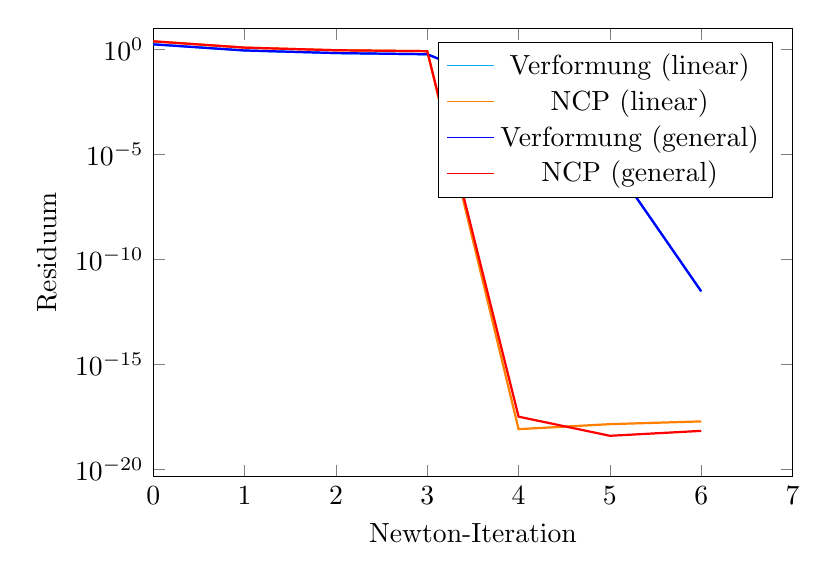
\begin{tikzpicture}[every plot/.append style={thick}] 
\begin{axis}[ 
label style={font=\normalsize}, 
xlabel={Newton-Iteration}, 
ylabel={Residuum}, 
xmin=0, xmax=7, 
ymode=log, 
ymin=0, ymax=10, 
width=0.8\textwidth, 
height=0.6\textwidth, 
legend pos=north east, 
legend style={cells={align=left}}, 
grid style=dashed, 
] 
\addplot[ 
color=cyan, 
] 
coordinates { 
(0, 1.71e+00)(1, 8.71e-01)(2, 6.55e-01)(3, 5.74e-01)(4, 1.02e-02)(5, 5.67e-06)(6, 2.89e-12)}; 
\addlegendentry{Verformung (linear)} 
\addplot[ 
color=orange, 
] 
coordinates { 
(0, 2.38e+00)(1, 1.19e+00)(2, 8.93e-01)(3, 8.06e-01)(4, 7.86e-19)(5, 1.36e-18)(6, 1.84e-18)}; 
\addlegendentry{NCP (linear)} 
\addplot[ 
color=blue, 
] 
coordinates { 
(0, 1.71e+00)(1, 8.71e-01)(2, 6.55e-01)(3, 5.74e-01)(4, 1.02e-02)(5, 5.67e-06)(6, 2.89e-12)}; 
\addlegendentry{Verformung (general)} 
\addplot[ 
color=red, 
] 
coordinates { 
(0, 2.38e+00)(1, 1.19e+00)(2, 8.93e-01)(3, 8.06e-01)(4, 3.09e-18)(5, 3.79e-19)(6, 6.51e-19)}; 
\addlegendentry{NCP (general)} 
\end{axis} 
\end{tikzpicture} 
\caption{Residuen des Stoffgesetzes 'Neo Hooke' mit Hinderniss 'Spitze' und 578 Freiheitsgraden für die Verschiebung.} 
\label{fiq:NeoHooke_Spitze_level3} 
\end{figure} 
